\documentclass{article}
\usepackage[utf8]{inputenc}
\usepackage{graphicx}

\title{CHAPTER 4}
\author{Dian Markuci (1184095)}
\date{24 November 2019}

\begin{document}

\maketitle

\section{TEORI}
\subsection{ Sejarah dan Contoh Pengelolaan File CSV}
Comma Separated Value atau CSV merupakan format data yang memudahkan penggunaanya dalam melakukan penginputan data ke database secara sederhana. CSV dapat digunakan dalam standar file ASCII, yang maksudnya setiap record dipisahkan dengan tanda(,) atau titik koma(;).File CSV digunakan untuk menyimpan informasi yang dipisahkan oleh koma, bukan menyimpan informasi dalam kolom.Dan jika teks dan angka disimpan dalam file csv maka mudah untuk memindahkannya dari satu program ke program lain. IBM Fortran (level H extended) compiler di bawah OS/360 mendukung fomat CSV pada tahun 1972. FORTRAN 77 mendefinisi penulisannya dimana input ataupun output menggunakan tanda koma atau spasi sebagai pembatas antar data dan penulisan tersebut sudah disetujui pada tahun 1978. Osborne Executive computer yang mengembangkan SuperCalc spreadsheet pada tahun 1983 membuat konvensi kutipan CSV yang memungkinkan string mengandung koma.\\

\textbf{Contoh}
\begin{center}
    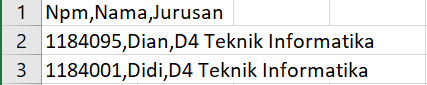
\includegraphics[width=8cm]{figure/contoh.png}
\end{center}

\subsection{Aplikasi Pembuat File CSV}
Ms.Excel, Google sheet, Notepad, dll

\subsection{Cara Menulis dan Membaca File CSV di Excel atau Spreadsheet}
\begin{enumerate}
    \item Buka Program Excel atau Spreadsheet Sejenis.
    \item Masukkan Data Pada Baris dan Kolom
    \item Save as, dan save file dengan format .csv
\end{enumerate}

\subsection{Library CSV}
\begin{center}
    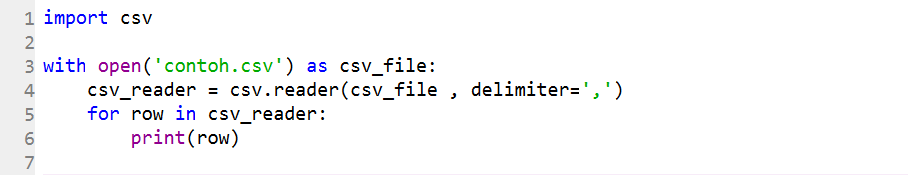
\includegraphics[width=8cm]{figure/1.png}
\end{center}

\begin{center}
    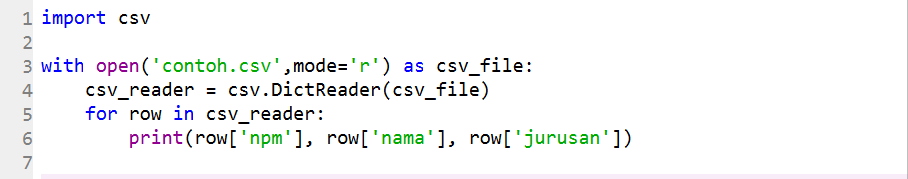
\includegraphics[width=8cm]{figure/2.png}
\end{center}

\begin{center}
    
\includegraphics[width=8cm]{figure/3.png}
\end{center}

\begin{center}
    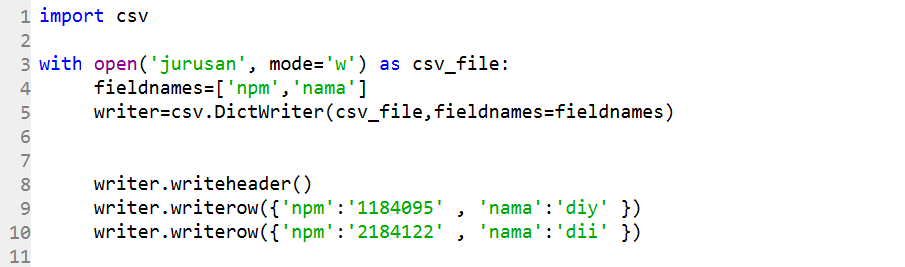
\includegraphics[width=8cm]{figure/4.png}
\end{center}

\subsection{Library Pandas}
\begin{center}
    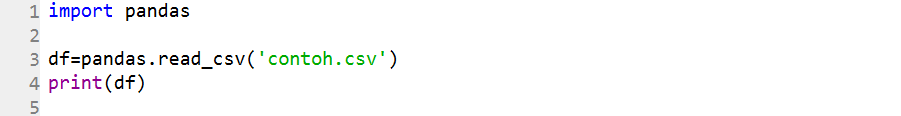
\includegraphics[width=8cm]{figure/pandas1.png}
\end{center}

\begin{center}
    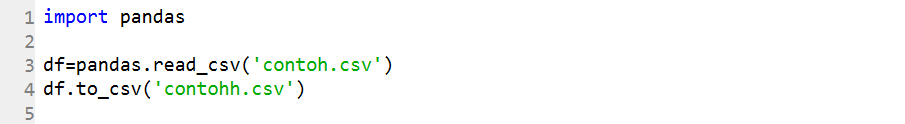
\includegraphics[width=8cm]{figure/pandas2.png}
\end{center}\\


\section{SOAL}

\begin{center}
    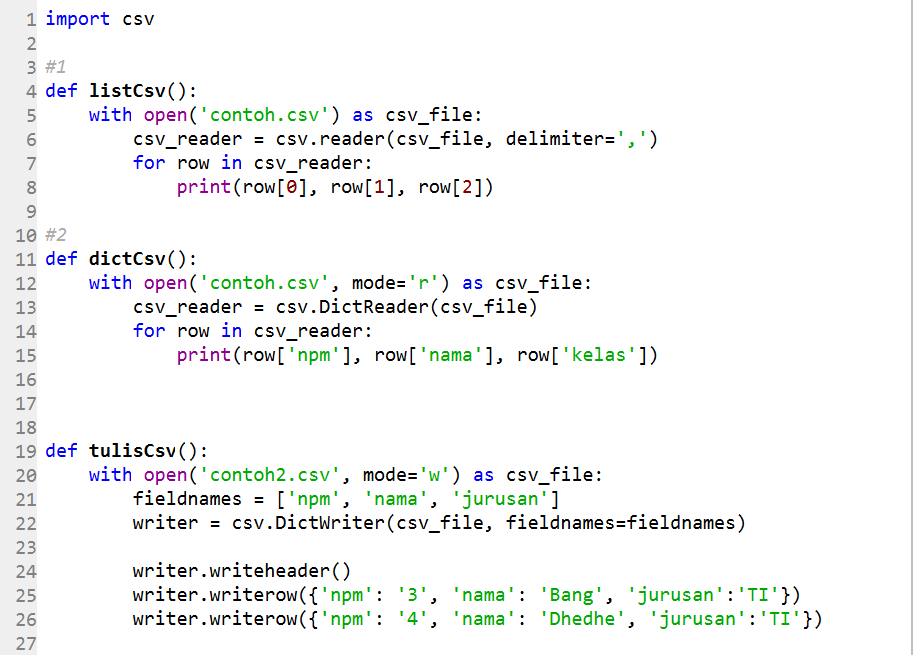
\includegraphics[width=8cm]{figure/soal1.png}
\end{center}
\begin{center}
    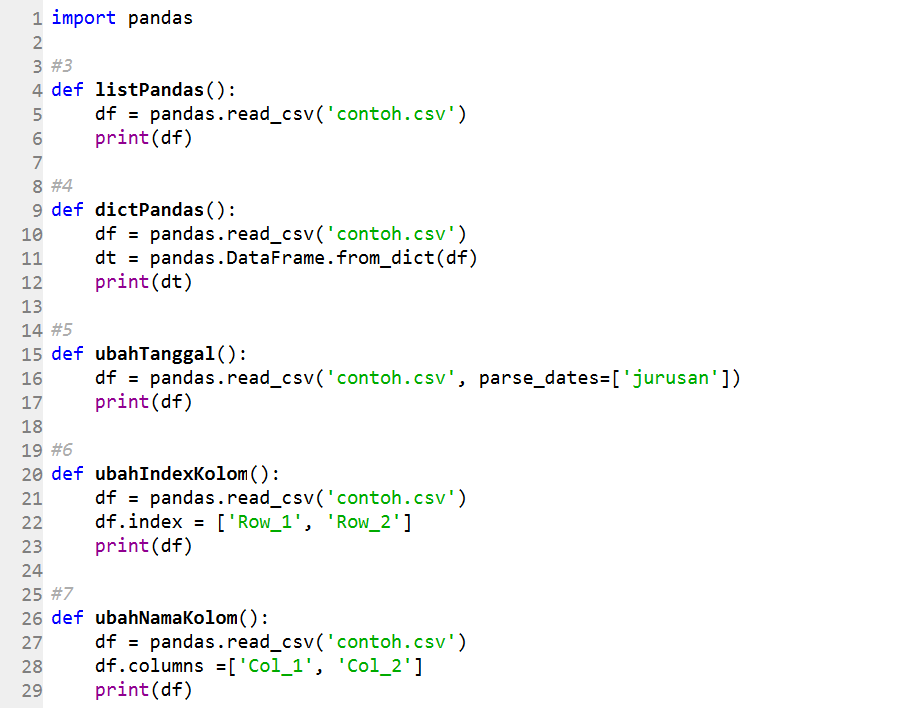
\includegraphics[width=8cm]{figure/soal2.png}
\end{center}
\begin{center}
    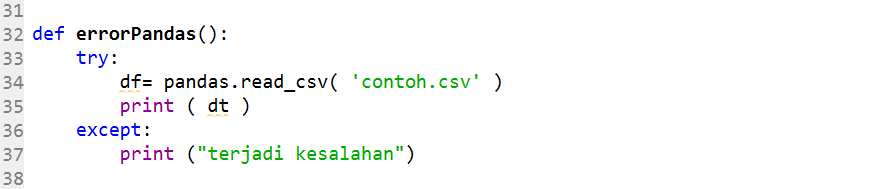
\includegraphics[width=8cm]{figure/soal3.png}
\end{center}





\end{document}
